\documentclass[../main.tex]{subfiles}

\graphicspath{{../images/}}

\usepackage[noend]{algpseudocode} % for pseudocode
\usepackage[plain]{algorithm} % float environment for algorithms
% preferred pseudocode style
\algrenewcommand{\algorithmicprocedure}{}
\algrenewcommand{\algorithmicthen}{}

% ``do { ... } while (cond)''
\algdef{SE}[DOWHILE]{Do}{doWhile}{\algorithmicdo}[1]{\algorithmicwhile\ #1}%

% ``for (x in y ... z)''
\newcommand{\ForRange}[3]{\For{#1 \textbf{in} #2 \ \ldots \ #3}}

\begin{document}
\pagestyle{fancy}
\chead{Lab 3}
\rhead{Junseo Shin}
\lhead{CSE 247}


\renewcommand{\thefigure}{\arabic{figure}}
\section*{Part 1: MergeSort}

\subsection*{Questions}

\begin{enumerate}
    \item PSEUDOCODE:
    \begin{algorithm}
        \caption{MergeSort BLOCKS}
        \begin{algorithmic}[1]
            \Procedure{\textbf{BLOCK 1}}{}
                \State $i++$
                \If{$i \bmod b = 0$}
                    \State \Call{read}{X, i, b}
                \EndIf
            \EndProcedure
            \Procedure{\textbf{BLOCK 2}}{}
                \State $j++$
                \If{$j \bmod b = 0$}
                    \State \Call{read}{Y, j, b}
                \EndIf
            \EndProcedure
        \end{algorithmic}
    \end{algorithm}

    \item The merge function must call the \texttt{read} and \texttt{write} functions
    $n/b$ times. 

    \section*{Part 2: Benchmarks}

    \item Bridges URL: \href{https://bridges-cs.herokuapp.com/assignments/247106/joonsuh}{https://bridges-cs.herokuapp.com/assignments/247106/joonsuh}
    \item Screenshots:
    % l3_4a.png and l3_4b.png
    \begin{figure}[ht]
        \centering
        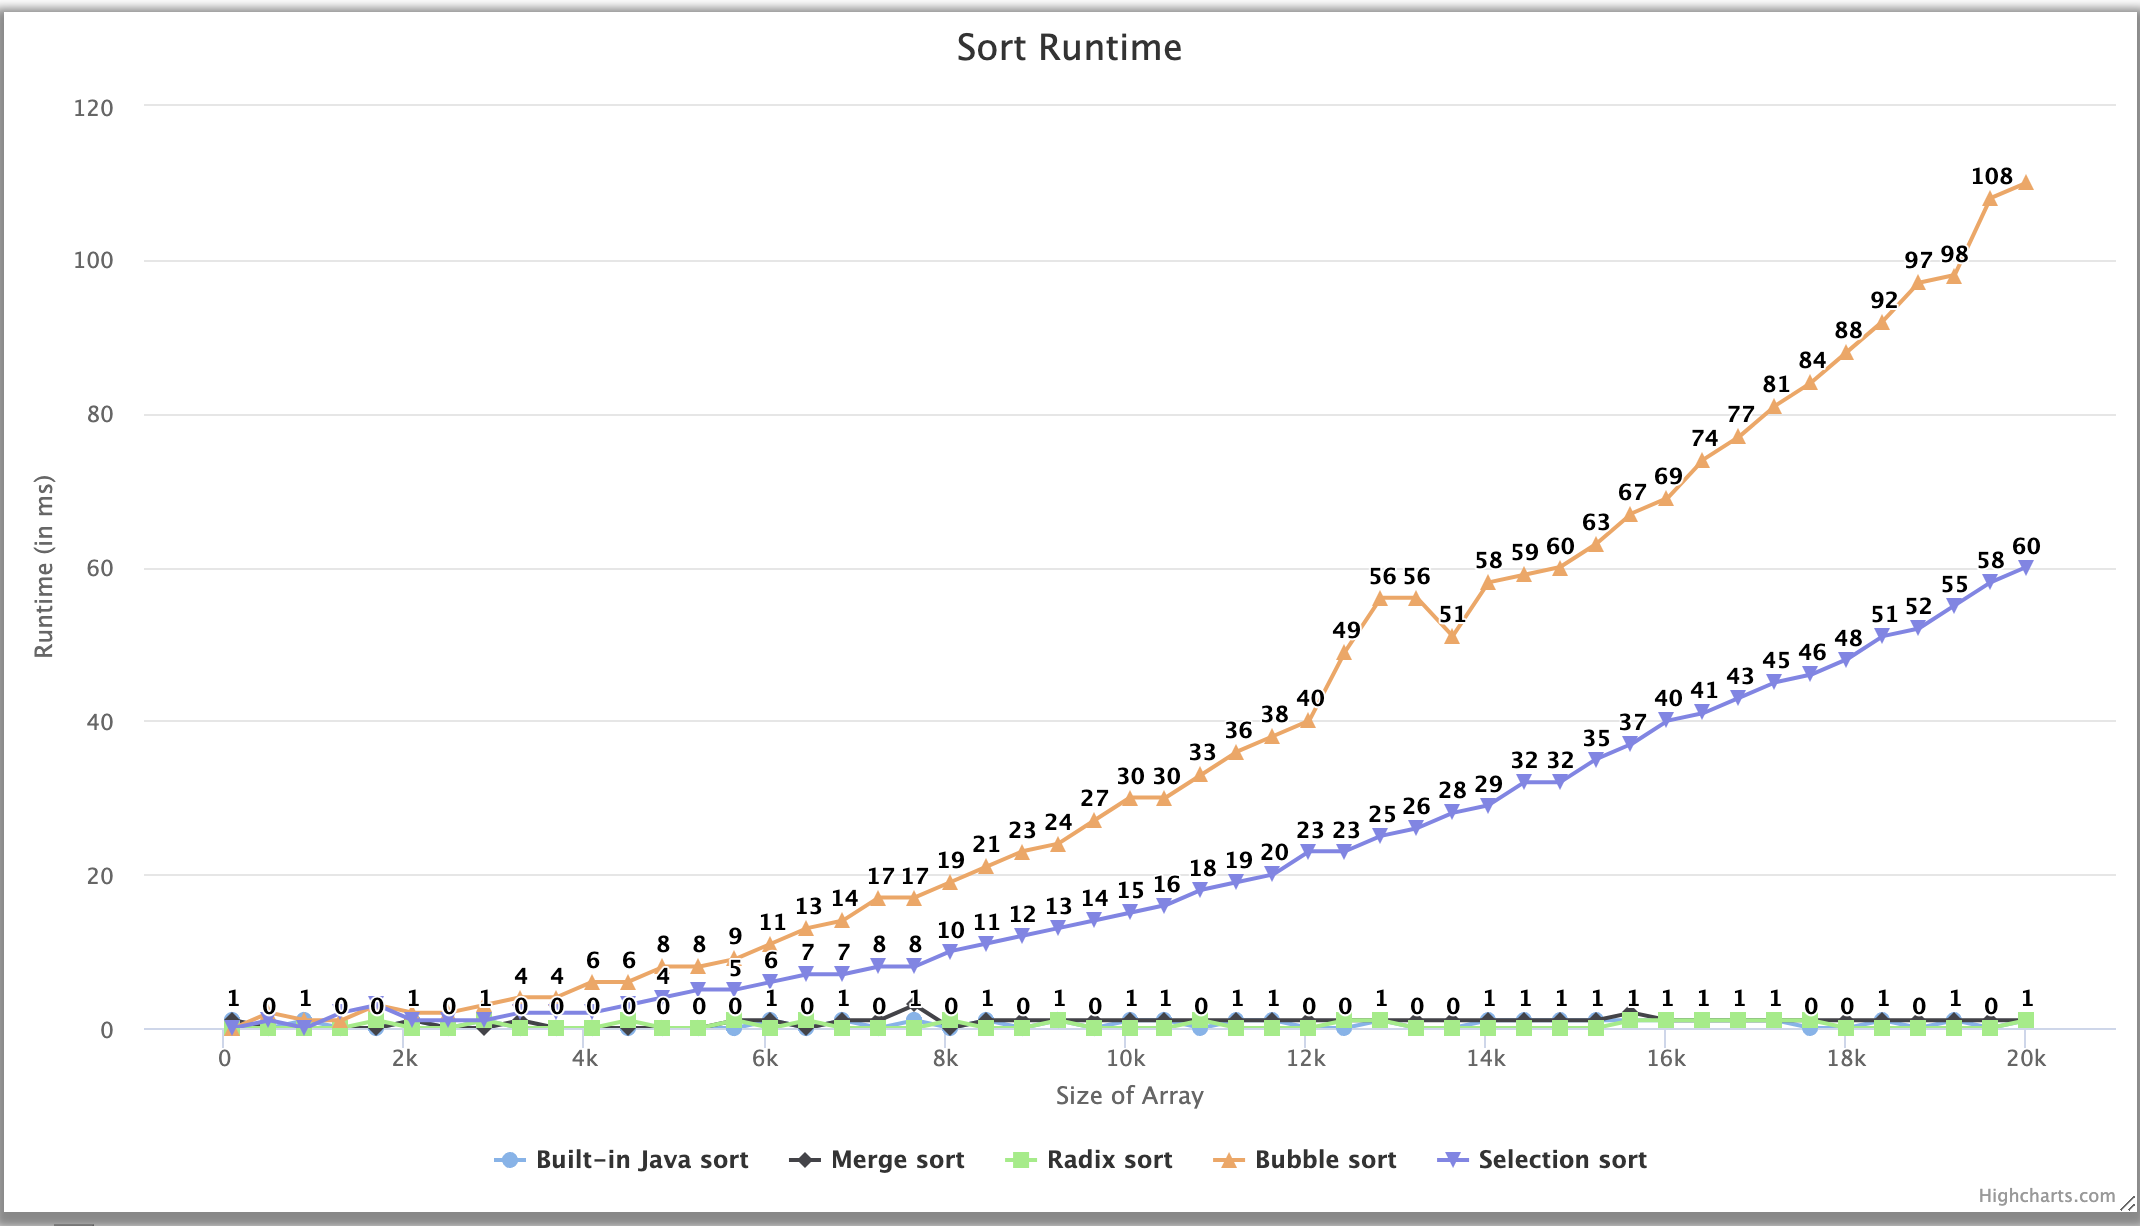
\includegraphics[width=0.8\textwidth]{l3_4a.png}
        \caption{Linearly scaled input graph}
        \label{fig:merge_sort}
    \end{figure}
    \begin{figure}[ht]
        \centering
        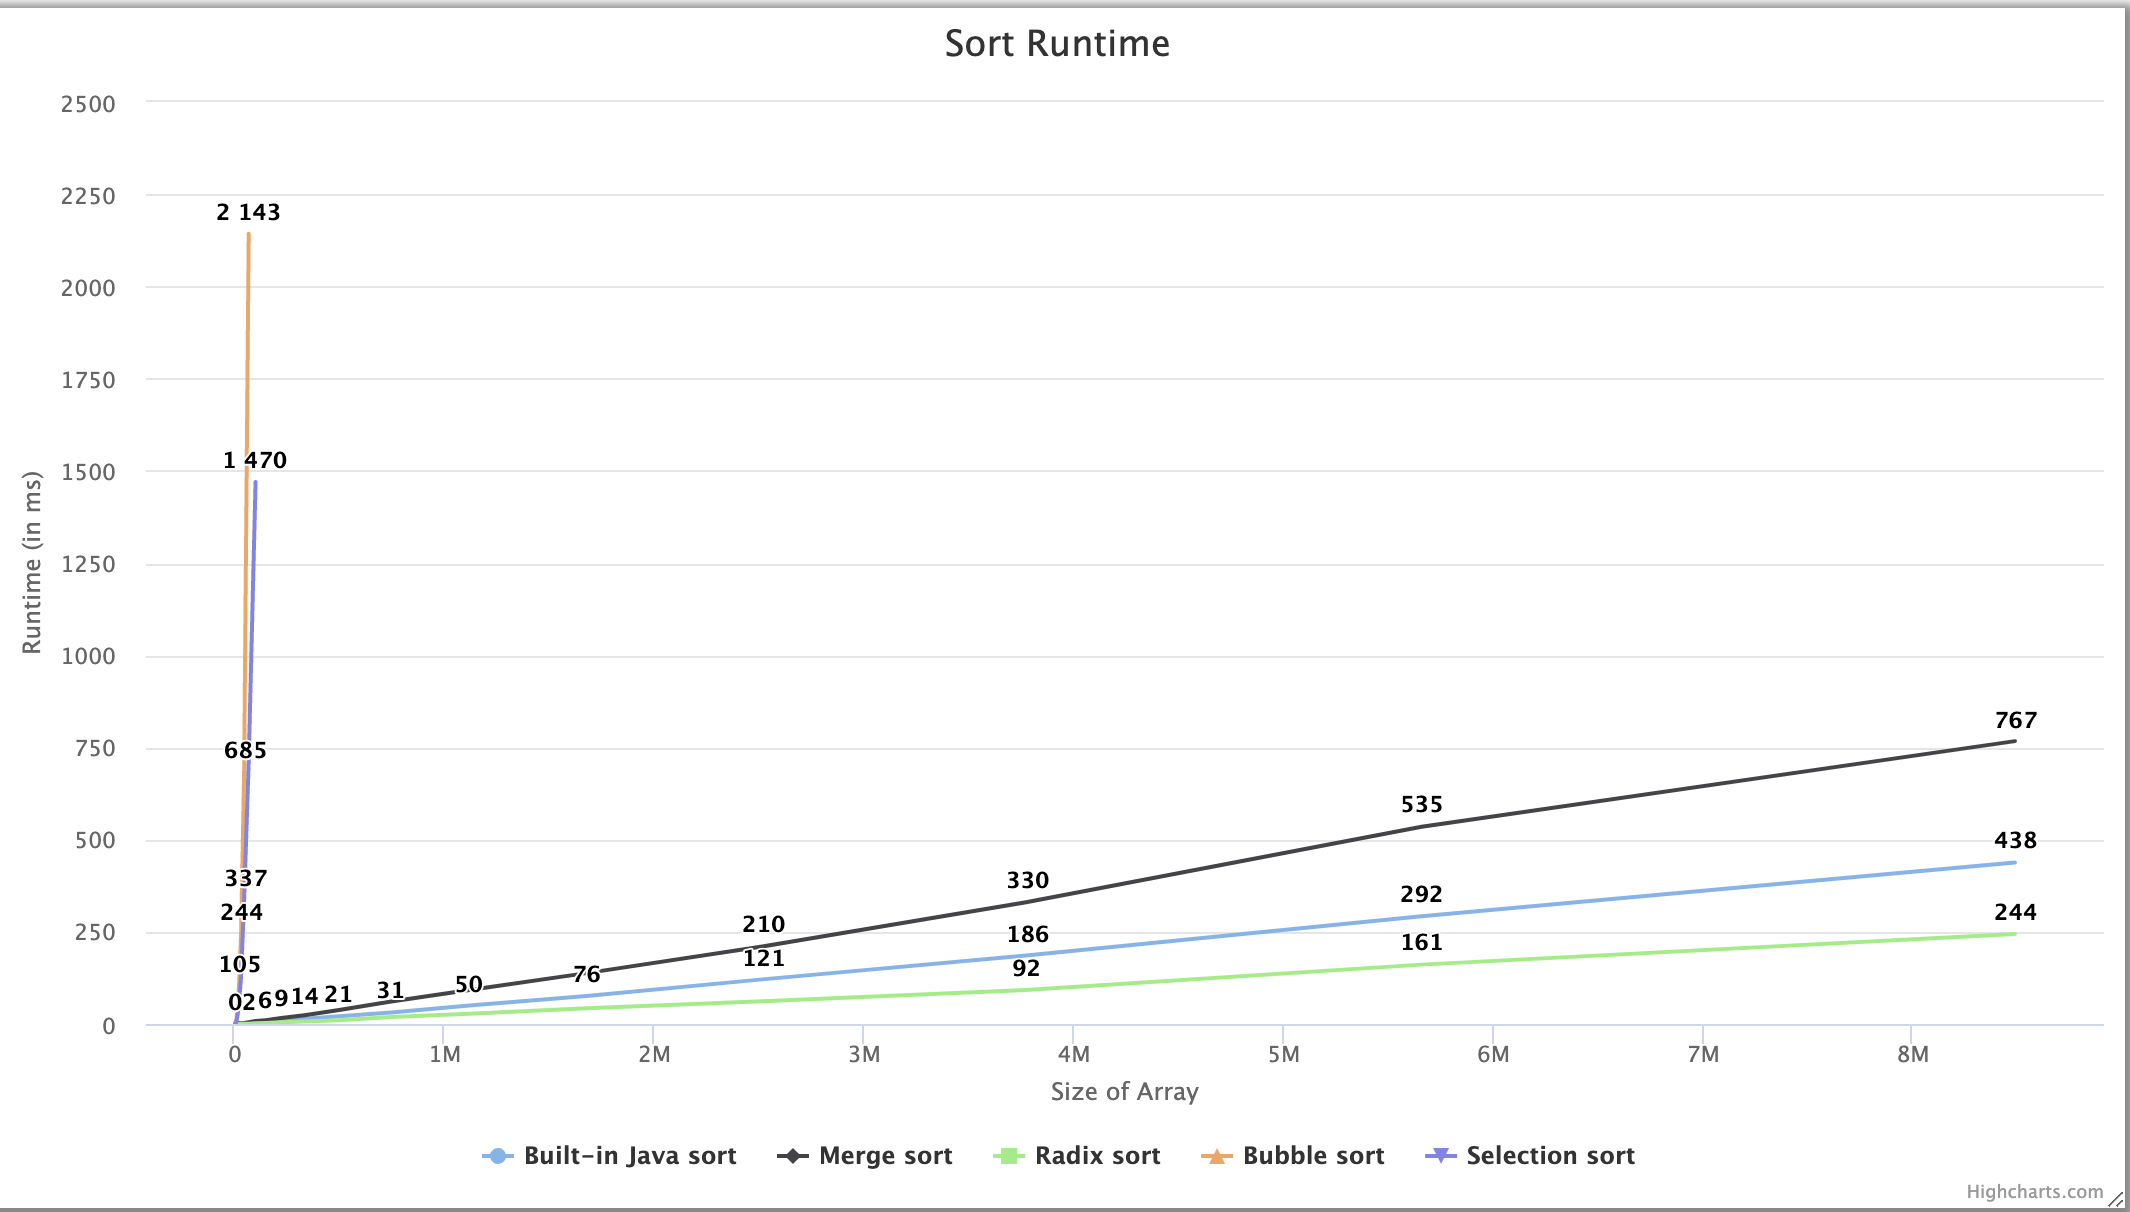
\includegraphics[width=0.8\textwidth]{l3_4b.png}
        \caption{Geometrically scaled input graph}
        \label{fig:merge_sort}
    \end{figure}

    \newpage
    \item From slowest to fastest the performance of the algorithms
    (selection sort, bubblesort, mergesort, radix sort) the performance of the algorithms is
    \begin{quote}
        selection sort $=$ bubblesort $\to$ mergesort $=$ built-in Java sort $\to$ radix sort
    \end{quote}

    \item When looking at selection sort and bubblesort, the performance of the algorithms is
    \begin{quote}
        bubblesort $\to$ selection sort
    \end{quote}
    where selection sort is slightly faster than bubblesort. Even though both algorithms have 
    $O(n^2)$ time complexity, selection sort is faster than bubblesort because it performs fewer
    swaps in total i.e. it only swaps the minimum element with the first element of the array vs.
    swapping adjacent elements in bubblesort.

\end{enumerate}




\end{document} 